\begin{figure*}[t!]
  \centering
  \definecolor{suscolor}{HTML}{4A90E2} % Gemini palette
  \definecolor{robcolor}{HTML}{E67E22} % Claude-Sonnet palette
  \definecolor{promptcolor}{HTML}{4A90E2}
  \definecolor{modelcolor}{HTML}{E67E22}
  \definecolor{ratingcolor}{HTML}{52B788}
  \definecolor{datacolor}{HTML}{F9E79F}
  \definecolor{susbgcolor}{HTML}{BDA0E3}
  \resizebox{0.7\textwidth}{!}{%
  \begin{tikzpicture}[
    font=\small,
    node distance=12mm and 18mm,
    % styles
    box/.style = {draw, rounded corners, inner sep=6pt, align=left},
    persona/.style = {draw=modelcolor!50!black, rounded corners=3pt, inner xsep=6pt, inner ysep=3pt, align=left, text=black, fill=modelcolor!25},
    title/.style = {font=\bfseries},
    arrow/.style = {line width=1pt, -{Latex[length=2.4mm,width=1.4mm]}},
  ]

  % Persona stack (center)
  \matrix (pers) [column sep=0mm, row sep=2mm] {
    \node[persona] (p0) {\faUser\ \ Persona $0$}; \\
    \node[persona] (p1) {\faUser\ \ Persona $1$}; \\
    \node[inner ysep=3pt, inner xsep=2pt] (dots) {$\vdots$}; \\
    \node[persona] (plast) {\faUser\ \ Persona $|\mathcal{P}|$}; \\
  };

  % Susceptibility box around personas (background layer so text stays visible)
  \begin{pgfonlayer}{background}
    \node[draw=susbgcolor!70!black, rounded corners, fill=susbgcolor!40,
          fit=(p0) (p1) (dots) (plast), inner xsep=12pt, inner ysep=10pt,
          label={[title]above:Moral Susceptibility},
          label={[text=black]below:Across-persona variability}] (susbox) {};
  \end{pgfonlayer}

  % Data block (vertical)
  \node[draw=black, rounded corners, inner xsep=6pt, inner ysep=6pt, align=center, fill=datacolor!70, label={[title]above:Model}] (modelbox) [left=32mm of susbox] {
    \begin{tikzpicture}[scale=0.42, line width=0.45pt]
      \foreach \y [count=\i] in {0.75,-0.35,-1.45} {
        \node[draw,circle,inner sep=1.2pt] (in\i) at (0,\y) {};
      }
      \foreach \y [count=\i] in {0.75,-0.35,-1.45} {
        \node[draw,circle,inner sep=1.2pt] (hid\i) at (1,\y) {};
      }
      \foreach \y [count=\i] in {0.2,-0.9} {
        \node[draw,circle,inner sep=1.2pt] (out\i) at (2,\y) {};
      }
      \foreach \i in {1,2,3} {
        \foreach \j in {1,2,3} {
          \draw (in\i) -- (hid\j);
        }
      }
      \foreach \i in {1,2,3} {
        \foreach \j in {1,2} {
          \draw (hid\i) -- (out\j);
        }
      }
    \end{tikzpicture}
  };

  \node[draw=black, rounded corners, inner xsep=6pt, inner ysep=6pt, align=left, fill=promptcolor!18, label={[title]above:Prompt}] (promptbox) [above=10mm of modelbox] {
    \begin{tabular}{@{}l@{}}
      \strut \faUser\ Persona\\[4pt]
      \strut \faFile\ MFQ
    \end{tabular}
  };

  \node[draw=black, rounded corners, inner xsep=6pt, inner ysep=6pt, align=center, fill=ratingcolor!22, label={[title]above:MFQ Scores}] (scorebox) [below=14mm of modelbox] {
    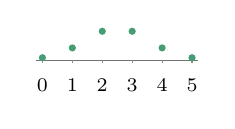
\begin{tikzpicture}[x=3.8mm, y=4.8mm, baseline=(current bounding box.center)]
      \draw[black!55] (-0.2,0) -- (5.2,0);
      \foreach \x/\y in {0/0.08,1/0.34,2/0.78,3/0.78,4/0.34,5/0.08} {
        \draw[black!45] (\x,0.03) -- (\x,-0.07);
        \fill[ratingcolor!85!black] (\x,\y) circle (1.3pt);
        \node[font=\scriptsize, below=2pt] at (\x,-0.07) {$\x$};
      }
    \end{tikzpicture}
  };

  \coordinate (promptarrowstart) at ($(promptbox.south)+(0,-8pt)$);
  \coordinate (modelarrowend) at ($(modelbox.north)+(0,8pt)$);
  \coordinate (modelarrowstart) at ($(modelbox.south)+(0,-13pt)$);
  \coordinate (scorearrowend) at ($(scorebox.north)+(0,13pt)$);
  \draw[arrow] (promptarrowstart) -- (modelarrowend);
  \draw[arrow] (modelarrowstart) -- (scorearrowend);

  % Robustness box (right)
  \node[
    box,
    draw=robcolor,
    text=black,
    fill=modelcolor!14,
    right=28mm of susbox,
    anchor=center,
    inner xsep=8pt,
    inner ysep=8pt,
    align=center
  ] (runs) {%
    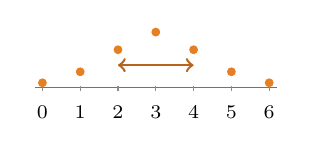
\begin{tikzpicture}[x=4.8mm, y=7mm, baseline=(current bounding box.center)]
      \draw[black!55] (-0.2,0) -- (6.2,0);
      \foreach \x/\y in {0/0.08,1/0.28,2/0.68,3/1.00,4/0.68,5/0.28,6/0.08} {
        \draw[black!45] (\x,0.03) -- (\x,-0.07);
        \fill[robcolor] (\x,\y) circle (1.6pt);
        \node[font=\scriptsize, below=2pt] at (\x,-0.07) {$\x$};
      }
      \draw[robcolor!80!black, line width=0.9pt, <->] (2,0.40) -- (4,0.40);
    \end{tikzpicture}
  };

  % Robustness title above runs
  \node[title, text=black, above=2mm of runs] {Moral Robustness};
  \node[text=black, below=2mm of runs] {Within-persona variability};

  % Merge point for persona arrows before entering robustness box
  \coordinate (merge) at ($(runs.center)+(-6mm,0)$);
  \coordinate (p0merge) at ($(p0.east)!0.60!(merge)$);
  \coordinate (p1merge) at ($(p1.east)!0.60!(merge)$);
  \coordinate (plastmerge) at ($(plast.east)!0.60!(merge)$);
  \coordinate (runsentry) at ($(runs.center)+(-1.5mm,0)$);

  % Persona arrows converge at merge point, leaving a small gap before merging
  \draw[arrow] (p0.east) -- (p0merge);
  \draw[arrow] (p1.east) -- (p1merge);
  \draw[arrow] (plast.east) -- (plastmerge);

  % Overall analysis grouping
  \coordinate (datatop) at ($(promptbox.north)+(0,6mm)$);
  \coordinate (databottom) at ($(scorebox.south)+(0,-6mm)$);

  \begin{pgfonlayer}{background}
    \node[draw=black, rounded corners, fit=(promptbox) (modelbox) (scorebox) (datatop) (databottom), inner xsep=8pt, inner ysep=0pt, label={[title]below:Data}] (databox) {};
    \node[draw=black, rounded corners, line width=0.9pt, fit=(susbox) (runs), inner xsep=28pt, inner ysep=26pt, label={[title]below:Benchmark}] (analysisbox) {};
  \end{pgfonlayer}


  \end{tikzpicture}%
  }% end \resizebox
  \caption{Left: summary of our data collection pipeline: we elicit models to respond to the MFQ conditioned on a persona. Right: summary of our benchmark pipeline: robustness, Eq.~\ref{eq:robustness}, and susceptibility, Eq.~\ref{eq:overall-susceptibility}, are computed from within and across persona variability in MFQ scores, respectively.}
  \label{fig:mfq-susceptibility-robustness}
\end{figure*}
